\chapter{滴定方法与曲线}\label{ch:b1:titration-methods}

一位药剂师收到一批标示
为 \qty{500}{mg} 的维生素 C 片，出售前须证明每片
确实含有标示的量。她不直接称量维生素，它与
黏合剂、填充剂混在一起，因此她采用滴定：
让它与已知浓度的试剂反应，测出所需体积，
再算出物质的量。用哪种反应、怎样看出终点、
结果有多可靠，这些正是本章要讨论的问题；本章把前五章
的平衡知识带到实验台上。

\begin{recall}
第 1 册（十一、十二年级）用颜色变化判断
酸被碱滴定的终点，用 pH 计与电导率仪跟踪滴定，
并使用等量关系 $C_AV_A = C_BV_B$。
预反应方法见\cref{ch:b1:predominant-reaction}；
沉淀、络合与氧化还原平衡见
\cref{ch:b1:precipitation,ch:b1:complexation,ch:b1:nernst}。
\end{recall}

\begin{omfigure}
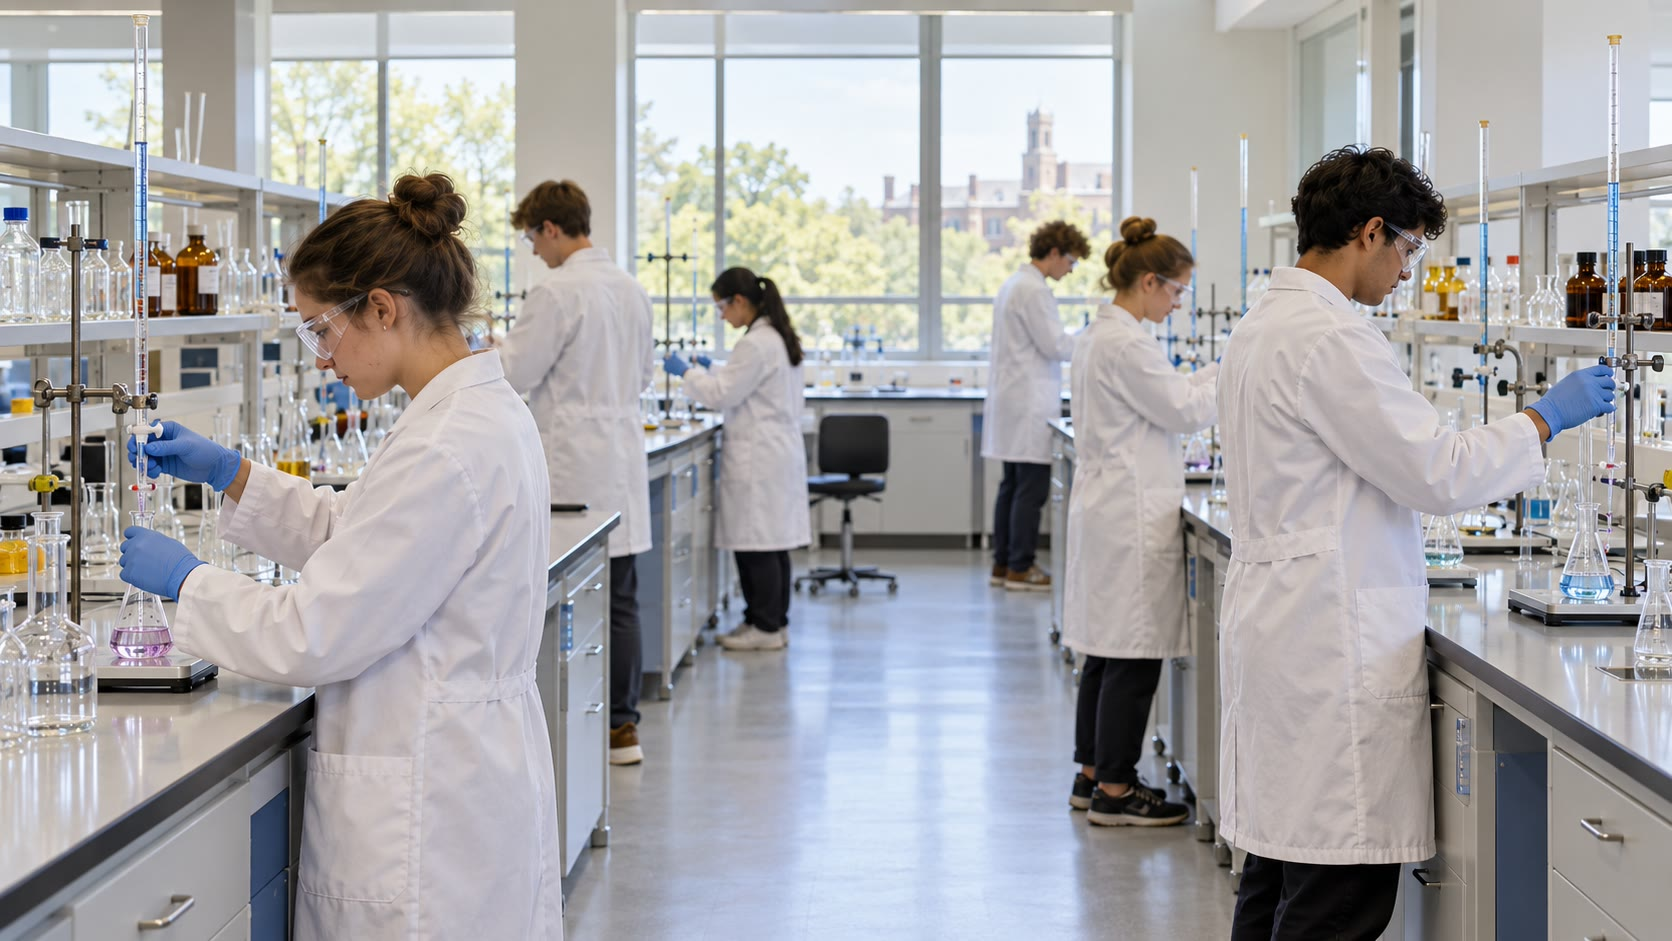
\includegraphics[width=0.66\linewidth]{images/book2/ai/b1-15-teaching-lab.jpg}

{\small 教学实验室：滴定管，磁力搅拌器上的锥形瓶，
手套与护目镜。滴定是化学中最常见的
定量测量方法。}
\end{omfigure}

\section{滴定与化学计量点}

\begin{definition}[滴定，化学计量点]\label{def:b1:titration-methods:titration}
\emph{滴定}\index{滴定}是通过使某物种（即\emph{待测物}\index{待测物}）与
已知浓度的试剂（即\emph{滴定剂}\index{滴定剂}）反应来测定其量的方法，滴定剂
被逐步加入。
反应必须单一、定量（$K$ 很大）且迅速。
\emph{化学计量点}\index{化学计量点}是指滴定剂与待测物
已按反应的化学计量比混合到一起的状态；此时所加体积即为
化学计量点体积，滴定曲线上该体积处的点
即为\emph{化学计量
点}\index{化学计量点}。实验者看到颜色变化或曲线出现转折时停止滴加，
此时的体积即为\emph{滴定
终点}\index{滴定终点}，好的方法应使终点与
化学计量点重合。
\end{definition}

\begin{proposition}[等量关系]\label{prop:b1:titration-methods:equivalence}
对于滴定反应 $a\,\mathrm{A} + b\,\mathrm{B} \to \cdots$，设待测物 A 的
物质的量为 $n_A$ 摩尔，滴定剂 B 的浓度为 $C_B$，
则化学计量点体积满足
\[
  \frac{n_A}{a} = \frac{C_B V_{\mathrm{eq}}}{b} .
\]
\end{proposition}

\begin{proof}
设 $x$ 为加入 $V$ 体积的滴定剂后的反应进度。化学计量点之前，
B 为限量试剂，反应定量进行，故 $x = C_BV/b$；化学计量点之后，
A 为限量试剂，$x = n_A/a$。化学计量点即两者同时耗尽的体积，
应同时满足 $n_A - ax = 0$ 与 $C_BV - bx = 0$，
消去 $x$ 即得该关系。
\end{proof}

\section{直接滴定与间接滴定}

\begin{definition}[滴定的类型]\label{def:b1:titration-methods:kinds}
在\emph{直接滴定}\index{直接滴定}中，滴定剂直接与待测物反应。
在\emph{返滴定}\index{返滴定}中，向待测物中加入已知过量的试剂，
再滴定剩余的试剂。若一份溶液含有多种待测物，
它们依次与滴定剂反应，则用\emph{连续滴定}\index{连续滴定}测定，
各化学计量点依次出现；
若它们一起反应、只给出一个化学计量点，
则用\emph{同时滴定}\index{同时滴定}测定，
所得结果
仅为它们的总和。
\end{definition}

\begin{method}[返滴定]\label{met:b1:titration-methods:back-titration}
适用于直接反应较慢、待测物不稳定或易挥发，
或没有指示剂适合直接反应时。
\begin{enumerate}
  \item 加入过量的试剂 R，其物质的量为 $n_R$，使其与待测物 A 完全反应
        （$\alpha\,\mathrm{A} + \rho\,\mathrm{R}$）。
  \item 用滴定剂 T（$\rho'\,\mathrm{R} +
        \tau\,\mathrm{T}$）滴定剩余的 R，至化学计量点时体积为 $V_T$。
  \item 计算 $n_{R,\text{过量}} = \frac{\rho'}{\tau}C_TV_T$，然后
        $n_A = \frac{\alpha}{\rho}(n_R - n_{R,\text{过量}})$。
\end{enumerate}
\end{method}

周末问题用这种方法滴定维生素 C：抗坏血酸还原过量的碘，
剩余的碘再用硫代硫酸盐滴定。

\section{pH 滴定与酸碱指示剂}

\begin{omfigure}
\begin{tikzpicture}[font=\small]
  \pic at (0,0) {stirrer};
  \pic at (0,0.18) {beaker={0.55}{omDef!14}};
  \pic at (0.2,2.45) {burette={0.75}{white}};
  \pic at (-0.45,0.45) {probe};
  \pic (m) at (-2.6,3.2) {meter={pH}};
  \draw[thick] (-0.45,3.45) to[out=90, in=0] (m-b);
  \node[anchor=west] at (0.65,6.2) {滴定管：NaOH，\qty{0.100}{mol/L}};
  \node[anchor=west] at (1.0,1.0) {酸，$V_0 = \qty{10.0}{mL}$，已稀释};
  \draw[<-, omProp, thick] (1.2,-0.25) -- (1.8,-0.25) node[anchor=west, text=black] {磁力搅拌器};
  \draw[<-, omProp, thick] (-0.62,2.4) -- (-1.5,2.0) node[anchor=east, text=black] {复合电极};
\end{tikzpicture}

{\small pH 滴定。复合玻璃电极在每次从滴定管加入滴定剂后
测量溶液的 pH；搅拌器使溶液混合。
电极事先用两种缓冲溶液校准。}
\end{omfigure}

\begin{omfigure}
\begin{tikzpicture}
\begin{axis}[name=s,
  width=0.5\linewidth, height=5.6cm, xmin=0, xmax=20, ymin=0, ymax=14,
  axis x line=bottom, axis y line=left, xlabel={$V$ (mL)}, ylabel={pH},
  xtick={0,5,10,15,20}, ytick={0,2,4,6,8,10,12,14},
  tick label style={font=\small}, label style={font=\small}]
\addplot[omDef, very thick] table[x=V, y=pH] {figdata/out/bachelor-1-titration-curves-strong.dat};
\addplot[omProp, thick] table[x=V, y=pH] {figdata/out/bachelor-1-titration-curves-weak.dat};
\node[font=\scriptsize, omDef, anchor=south west] at (axis cs:6,0.2) {盐酸 \ce{HCl}};
\node[font=\scriptsize, omProp, anchor=west] at (axis cs:0.4,6.4) {乙酸 \ce{CH3COOH}};
\draw[dotted] (axis cs:5,0) -- (axis cs:5,4.76) -- (axis cs:0,4.76);
\node[font=\scriptsize, anchor=north] at (axis cs:2.5,4.7) {$\mathrm{p}K_a$};
\end{axis}
\begin{axis}[at={(s.east)}, anchor=west, xshift=1.2cm,
  width=0.5\linewidth, height=5.6cm, xmin=0, xmax=20, ymin=0, ymax=14,
  axis x line=bottom, axis y line=left, xlabel={$V$ (mL)}, ylabel={pH},
  xtick={0,5,10,15,20}, ytick={0,2,4,6,8,10,12,14},
  tick label style={font=\small}, label style={font=\small}]
\addplot[omMeth, very thick] table[x=V, y=pH] {figdata/out/bachelor-1-titration-curves-mixture.dat};
\node[font=\scriptsize, anchor=west, align=left] at (axis cs:10.8,6.0) {\ce{HCl} + \ce{CH3COOH}\\ 两个等当点};
\end{axis}
\end{tikzpicture}

{\small 左图：\qty{10.0}{mL} 盐酸和乙酸，
二者浓度均为 \qty{0.100}{mol/L}，用
\qty{0.100}{mol/L} 氢氧化钠溶液滴定。弱酸在半等当点处 pH $=
\mathrm{p}K_a$，化学计量点的 pH 为 8.73。
右图：混合物，每种酸的浓度均为 \qty{0.050}{mol/L}，
先滴定强酸（等当点在 \qty{5}{mL}），再滴定
弱酸（\qty{10}{mL}）。}
\end{omfigure}

\begin{proposition}[弱酸的半等当点]\label{prop:b1:titration-methods:half-equivalence}
用强碱滴定弱酸 HA 时，在半等当点处
$\mathrm{pH} = \mathrm{p}K_a$，前提是酸既不太强，
也不太稀（$\mathrm{p}K_a$ 大致在 4 到 10 之间，
浓度为 \qty{0.1}{mol/L} 时）。
\end{proposition}

\begin{proof}
在半等当点处，定量反应 \ce{HA + OH- -> A- + H2O}
已将一半 HA 转化，即 $[\mathrm{HA}] = [\mathrm{A^-}]$，
由亨德森关系式可得 $\mathrm{pH} = \mathrm{p}K_a$。该条件
保证 HA 与水的反应以及 $\mathrm{A^-}$ 与水的反应
不会明显改变这些物质的量。
\end{proof}

\begin{proposition}[弱酸化学计量点处的 pH]\label{prop:b1:titration-methods:ph-at-equivalence}
用强碱滴定弱酸（$\mathrm{p}K_a$）至化学计量点时，
溶液为共轭碱，浓度为 $C'$（稀释后），且
\[
  \mathrm{pH} = \tfrac12(\mathrm{p}K_e + \mathrm{p}K_a + \log C') .
\]
\end{proposition}

\begin{proof}
碱与水的主反应
\ce{A- + H2O <=> HA + OH-}，其 $K = K_e/K_a$；碱的转化量很小，
$[\ce{OH-}] = \sqrt{KC'}$（见\cref{prop:b1:predominant-reaction:ph-formulas}），
由此得到结果。对乙酸而言，$C' = \qty{0.050}{mol/L}$，
于是 $\frac12(14.00 + 4.76 - 1.30) = 8.73$。
\end{proof}

\begin{proposition}[连续滴定]\label{prop:b1:titration-methods:successive}
两种酸用同一碱滴定时，各自的等当点可以分别给出，
误差小于 \qty{1}{\percent}，前提是它们的 $\mathrm{p}K_a$ 相差至少为 4。
\end{proposition}

\begin{proof}
在第一个等当点处，碱 $\mathrm{A_1^-}$ 与
第二种酸 $\mathrm{HA_2}$ 的反应 $\mathrm{A_1^-} + \mathrm{HA_2}
\rightleftharpoons \mathrm{HA_1} + \mathrm{A_2^-}$ 的 $K = 10^{\mathrm{p}K_1 - \mathrm{p}K_2}$。
设起始两者物质的量相等，第二种酸已被滴定的分数 $x$
满足 $x^2/(1 - x)^2 = K$；当 $x \leqslant 0.01$ 时，$K
\leqslant 10^{-4}$，即 $\mathrm{p}K_2 - \mathrm{p}K_1 \geqslant 4$。
\end{proof}

磷酸（2.15、7.21、12.34）给出两个清晰的等当点；第三个
等当点在碱的水中被掩盖。乙酸与盐酸的混合物
（见图右侧）在其后被滴定，强酸实际上
相当于 $\mathrm{p}K_a$ 小于 0 的酸。

\begin{method}[由曲线确定等当点]\label{met:b1:titration-methods:derivative}
\begin{enumerate}
  \item 微商法：计算相邻各点之间的 $\Delta\mathrm{pH}/\Delta V$，
        等当点处该比值最大。
  \item 切线法：在突跃两侧各作曲线的一条切线，两者
        互相平行；再作与二者等距的平行线，它与曲线
        的交点即为化学计量点。
\end{enumerate}
\end{method}

\begin{method}[切线法（计算）]\label{met:b1:titration-methods:tangents}
对由计算机记录的曲线，将突跃每一侧的数据点
用光滑函数拟合，并取拐点；对于
对称突跃（强酸、强碱），突跃中点位于
pH 为 7 处，即为化学计量点。
\end{method}

\begin{definition}[显色指示剂，变色区间]\label{def:b1:titration-methods:indicator}
\emph{显色指示剂}\index{显色指示剂}是弱酸碱对
HIn/In$^-$，其两种形式颜色不同。其颜色
在\emph{变色区间}\index{变色区间}内发生改变，即两种形式都不占明显优势的
pH 范围，约为 $\mathrm{p}K_{a}(\mathrm{HIn}) \pm 1$。
\end{definition}

\begin{omfigure}
\begin{tabular}{lccl}
\hline
指示剂 & $\mathrm{p}K_a$ & 变色区间 & 颜色（酸式 / 碱式） \\
\hline
甲基橙 & 3.5 & 2.5--4.5 & 红 / 黄 \\
甲基红 & 4.8 & 3.8--5.8 & 红 / 黄 \\
酚红 & 7.9 & 6.9--8.9 & 黄 / 红 \\
百里酚蓝（第二次变色） & 9.2 & 8.2--10.2 & 黄 / 蓝 \\
\hline
\end{tabular}

\smallskip
{\small 四种指示剂，$\mathrm{p}K_a$ 取自经审校的
解离常数汇编；变色区间为 $\mathrm{p}K_a \pm 1$。}
% ledger: pka:methylorange, pka:methylred, pka:phenolred, pka:thymolblue2
\end{omfigure}

\begin{method}[选择指示剂]\label{met:b1:titration-methods:choose-indicator}
选择变色区间位于曲线竖直突跃之内的指示剂，
并尽量接近化学计量点时的 pH。强酸被强碱滴定
（此处 $\pm\qty{0.1}{mL}$ 时突跃为 3.3 至 10.7）：四种均可。
乙酸（化学计量点为 8.73）：宜用酚红或百里酚蓝；甲基橙
会在远早于化学计量点时就变色。
\end{method}

\section{电位滴定}

\begin{definition}[电位滴定]\label{def:b1:titration-methods:potentiometric}
\emph{电位滴定}\index{电位滴定}是指在滴定过程中跟踪溶液中某电极
相对于参比电极的电势，适用于氧化还原（铂丝）、
沉淀（银丝）或配位
滴定。
\end{definition}

\begin{proposition}[氧化还原滴定的特征点]\label{prop:b1:titration-methods:potentiometric-points}
对 $\mathrm{Red_1}$ 用 $\mathrm{Ox_2}$ 滴定，其反应为
$n_2\,\mathrm{Red_1} + n_1\,\mathrm{Ox_2} \to n_2\,\mathrm{Ox_1} +
n_1\,\mathrm{Red_2}$（分别转移 $n_1$ 和 $n_2$ 个电子的电对），$E(V_{\mathrm{eq}}/2) = E^\circ_1$，$E(2V_{\mathrm{eq}}) =
E^\circ_2$，化学计量点时
\[
  E_{\mathrm{eq}} = \frac{n_1E^\circ_1 + n_2E^\circ_2}{n_1 + n_2},
\]
对于半反应中不涉及其他物种的电对（或在
使额外项保持不变的 pH 下）。
\end{proposition}

\begin{proof}
在半等当点时，$\mathrm{Red_1}$ 的一半被氧化：
$[\mathrm{Ox_1}] = [\mathrm{Red_1}]$，由电对 1 的能斯特方程
可得 $E^\circ_1$。当 $2V_{\mathrm{eq}}$ 时，过量的 $\mathrm{Ox_2}$
与被还原的量相等：$[\mathrm{Ox_2}] = [\mathrm{Red_2}]$，$E = E^\circ_2$。
在化学计量点时，将电对 1 的能斯特方程乘以 $n_1$，电对 2 的乘以 $n_2$，
再相加；化学计量关系使
$[\mathrm{Ox_1}]/[\mathrm{Red_1}] \cdot [\mathrm{Ox_2}]/[\mathrm{Red_2}] = 1$
（剩余的 $\mathrm{Red_1}$ 与 $\mathrm{Ox_2}$ 的量
与生成物之比相同），因此对数项相消。
\end{proof}

在 \qty{1}{mol/L} 酸中以高锰酸盐滴定铁(II)时，$n_1 = 1$ 且 $n_2 =
5$：$E_{\mathrm{eq}} = (0.77 + 5 \times 1.51)/6 = 1.39$~V。突跃从
约 0.8 至 1.5~V，突跃很大，终点十分明显；实际上
高锰酸盐本身即为指示剂，其紫色
在过量第一滴时即持续不褪。

\begin{omfigure}
\begin{tikzpicture}
\begin{axis}[name=p,
  width=0.5\linewidth, height=5.6cm, xmin=0, xmax=20, ymin=0.6, ymax=1.6,
  axis x line=bottom, axis y line=left, xlabel={$V$ (mL)}, ylabel={$E$ (V)},
  xtick={0,5,10,15,20},
  tick label style={font=\small}, label style={font=\small}]
\addplot[omDef, very thick] table[x=V, y=E] {figdata/out/bachelor-1-titration-curves-potentiometric.dat};
\draw[dotted] (axis cs:5,0.6) -- (axis cs:5,0.77) -- (axis cs:0,0.77);
\draw[dotted] (axis cs:10,0.6) -- (axis cs:10,1.39) -- (axis cs:0,1.39);
\node[font=\scriptsize, anchor=south west] at (axis cs:0.2,0.77) {0.77};
\node[font=\scriptsize, anchor=south west] at (axis cs:0.2,1.39) {1.39};
\end{axis}
\begin{axis}[at={(p.east)}, anchor=west, xshift=1.2cm,
  width=0.5\linewidth, height=5.6cm, xmin=0, xmax=20, ymin=0, ymax=4.6,
  axis x line=bottom, axis y line=left, xlabel={$V$ (mL)},
  ylabel={$\kappa$ (mS/cm)}, xtick={0,5,10,15,20},
  tick label style={font=\small}, label style={font=\small}]
\addplot[omProp, very thick] table[x=V, y=kappa] {figdata/out/bachelor-1-titration-curves-conductimetric.dat};
\draw[dotted] (axis cs:10,0) -- (axis cs:10,1.15);
\end{axis}
\end{tikzpicture}

{\small 左图：电位滴定 \qty{10.0}{mL} 铁(II)溶液（浓度为
\qty{0.100}{mol/L}），以浓度为 \qty{0.0200}{mol/L} 的高锰酸盐滴定，
在 \qty{1}{mol/L} 的酸中进行（铂电极，电势相对于氢
电极）。右图：电导滴定 \qty{100}{mL} 的盐酸，浓度为
\qty{0.0100}{mol/L}，以氢氧化钠滴定，其浓度为
\qty{0.100}{mol/L}；化学计量点位于两条
直线的交点处。}
% ledger: lam:H+, lam:OH-, lamsalt:HCl, lamsalt:NaCl (conductivities in figdata/bachelor-1/titration-curves.py)
\end{omfigure}

\section{电导滴定、配位滴定和沉淀滴定}

\begin{definition}[离子摩尔电导率]\label{def:b1:titration-methods:conductivity}
溶液的电导率 $\kappa$（单位为 \unit{S/m}）衡量其
借离子运动传导电流的能力。称\emph{离子摩尔
电导率}\index{离子摩尔电导率} $\lambda_i$ 为该离子的
单位体积、每摩尔的导电贡献；其无限稀释时的值
$\lambda_i^\circ$ 是该离子与溶剂在给定
温度下的常数。
\end{definition}

\begin{proposition}[科尔劳施定律]\label{prop:b1:titration-methods:kohlrausch}
稀溶液中，电导率为各
离子贡献之和：
\[
  \kappa = \sum_i \lambda_i^\circ c_i ,
\]
\emph{科尔劳施定律}\index{科尔劳施定律}：盐的摩尔电导率
等于其所含各离子摩尔电导率之和。
\end{proposition}

\admitted{科尔劳施定律表明，稀溶液中离子各自独立运动；
其在较高浓度下的适用限度，在
本科二年级分册中研究。这里将其作为实验定律使用。}

\begin{proposition}[电导滴定的斜率]\label{prop:b1:titration-methods:conductimetric-slopes}
用强碱滴定强酸 H$^+$X$^-$ 时，
即以 Na$^+$OH$^-$ 为滴定剂（忽略稀释，体积很大），电导率
随所加体积线性变化，斜率在化学计量点前与
$\lambda^\circ(\ce{Na+}) - \lambda^\circ(\ce{H+}) < 0$ 成正比，
在化学计量点后与 $\lambda^\circ(\ce{Na+}) + \lambda^\circ(\ce{OH-}) > 0$
成正比。
\end{proposition}

\begin{proof}
化学计量点前，每加入一摩尔氢氧根离子，便消耗一摩尔
\ce{H+}（\ce{H+ + OH- -> H2O}），并引入一摩尔 \ce{Na+}；化学计量点后，
则加入一个 \ce{Na+} 和一个 \ce{OH-}。\ce{X-} 不变。
由科尔劳施定律可知，电导率的变化为这些
$\lambda^\circ$ 的组合乘以所加物质的量，再除以（固定的）体积。
\end{proof}

由极限电导率 $\lambda^\circ(\ce{H+}) =
\qty{349.8}{S.cm^2/mol}$、$\lambda^\circ(\ce{OH-}) = 198.3$，以及盐
\ce{HCl}（426）和 \ce{NaCl}（126.5）的数值，由科尔劳施定律可得
$\lambda^\circ(\ce{Cl-}) = 426 - 349.8 = 76.2$，$\lambda^\circ(\ce{Na+}) =
126.5 - 76.2 = 50.3$~\unit{S.cm^2/mol}。氢离子和氢氧根离子
的导电能力远强于其他离子：曲线呈尖锐的 V 形。

配位滴定使用 EDTA：在 pH 10（氨缓冲溶液）中，钙离子
和镁离子均与之定量反应（条件常数见
\cref{ch:b1:complexation}），若某指示剂本身是该金属的弱配位剂，
当 EDTA 夺取其中最后的金属离子时，指示剂变色——
水的硬度滴定即属此类。
沉淀滴定使用银离子：以硝酸银滴定氯离子，
以铬酸根为指示剂（见\cref{exo:b1:precipitation:8}），或
用银电极跟踪（见\cref{ch:b1:nernst}）。这些结果的精度
由玻璃仪器和滴定终点决定，
在\cref{ch:b1:lab-techniques-1}中讨论。

\section{练习}

\begin{exercise}[$\star$]\label{exo:b1:titration-methods:1}
\qty{20.0}{mL} 氢氧化钠溶液，恰好需要 \qty{12.4}{mL}
浓度为 \qty{0.100}{mol/L} 的盐酸。写出反应式及其平衡常数，
并计算碱的浓度。
\end{exercise}

\begin{exercise}[$\star$]\label{exo:b1:titration-methods:2}
表中哪种指示剂适用于以 \qty{0.10}{mol/L} 盐酸滴定氨水（\qty{0.10}{mol/L}，
$\mathrm{p}K_a = 9.25$）？请先计算
化学计量点的 pH。
\end{exercise}

\begin{exercise}[$\star$]\label{exo:b1:titration-methods:3}
用 \qty{0.0200}{mol/L} 的高锰酸钾滴定 \qty{10.0}{mL} 亚铁离子，
紫色自 \qty{12.6}{mL} 起持续不褪。
写出反应式，并计算亚铁离子的浓度。
\end{exercise}

\begin{exercise}[$\star$]\label{exo:b1:titration-methods:4}
取 \qty{50.0}{mL} 水样，在 pH 10 下，用
\qty{0.0100}{mol/L} 的 EDTA 滴定，化学计量点在 \qty{14.2}{mL} 处。
EDTA 与钙离子、镁离子均按一比一反应，计算
这两种离子的总浓度。这是同时滴定
还是连续滴定？
\end{exercise}

\begin{exercise}[$\star\star$]\label{exo:b1:titration-methods:5}
对 \qty{10.0}{mL}、\qty{0.100}{mol/L} 的乙酸，
以 \qty{0.100}{mol/L} 的氢氧化钠滴定，计算加入 0、5.0、10.0
和 \qty{15.0}{mL} 碱时的 pH（用\cref{ch:b1:predominant-reaction}中的方法），
并与本章曲线比较。
\end{exercise}

\begin{exercise}[$\star\star$]\label{exo:b1:titration-methods:6}
证明用氢氧化钠滴定磷酸的 pH 滴定曲线
出现两个突跃，并计算酸浓度为 \qty{0.100}{mol/L} 时每个化学计量点的
pH（取 \qty{10.0}{mL} 酸，碱浓度 \qty{0.100}{mol/L}）。为何不出现
第三个突跃？
\end{exercise}

\begin{exercise}[$\star\star$]\label{exo:b1:titration-methods:7}
盐酸与乙酸的混合液（\qty{10.0}{mL}）用
\qty{0.100}{mol/L} 的氢氧化钠滴定，出现两个化学计量点，分别在
\qty{6.2}{mL} 和 \qty{14.6}{mL} 处。计算两种酸的浓度。
求两个化学计量点中间（即半途）的 pH。
\end{exercise}

\begin{exercise}[$\star\star$]\label{exo:b1:titration-methods:8}
计算用高锰酸钾滴定亚铁离子时铂电极的电势
（使用本章数据），加入 2.0、9.0、11.0 和
\qty{20.0}{mL} 滴定剂时的电势。
\end{exercise}

\begin{exercise}[$\star\star$]\label{exo:b1:titration-methods:9}
利用科尔劳施定律和本章数据，计算用碱滴定盐酸时，
加入 0、10.0 和 \qty{20.0}{mL} 碱时，被滴盐酸的电导率
（取 \qty{100}{mL}、\qty{0.0100}{mol/L} 的酸，碱浓度
\qty{0.100}{mol/L}，计入稀释），并求两段斜率。
\end{exercise}

\begin{exercise}[$\star\star\star$]\label{exo:b1:titration-methods:10}
证明忽略稀释时，强碱滴定强酸的 pH 滴定曲线
关于化学计量点对称，并计算本章滴定在
$V_{\mathrm{eq}} \pm 0.1$~mL 之间的突跃大小。若所有
浓度都除以 100，
突跃将如何变化？
\end{exercise}

\begin{exercise}[$\star\star\star$]\label{exo:b1:titration-methods:11}
推导用高锰酸钾滴定亚铁离子时电位滴定曲线的方程，
分别给出化学计量点前后的表达式，并核对
\cref{prop:b1:titration-methods:potentiometric-points}中的三个特殊点。
在 pH 1 时，化学计量点的电势将如何变化？
\end{exercise}

\begin{exercise}[$\star\star\star$]\label{exo:b1:titration-methods:12}
氯化铵（\qty{0.100}{mol/L}，$\mathrm{p}K_a = 9.25$）不能用指示剂
由氢氧化钠准确滴定。试由曲线说明原因，然后设计一个返滴定方案：
加入过量氢氧化钠，煮沸除去氨，
再用盐酸滴定剩余的氢氧根。
写出计算过程。
\end{exercise}

\section{问题：药片中有多少维生素 C？}

\begin{problem}[{周末问题——碘与抗坏血酸的反应，
硫代硫酸钠返滴定，结果的计算，
及其不确定度，最后求每片药片中抗坏血酸的质量}]
\label{pb:b1:titration-methods:1}
将一片药片研碎后溶于水中，转移至 \qty{100.0}{mL}
容量瓶中。用移液管取 \qty{10.00}{mL} 试液，
加入 \qty{20.00}{mL} 浓度为 \qty{0.0250}{mol/L} 的碘溶液（过量）。剩余的碘
用浓度为 \qty{0.0500}{mol/L} 的硫代硫酸钠溶液滴定，以淀粉为指示剂，
蓝色在 \qty{8.90}{mL} 时消失。
抗坏血酸为 \ce{C6H8O6}（$M = \qty{176.0}{g/mol}$）；碘将其
氧化为 \ce{C6H6O6}。$E^\circ(\ce{I2}/\ce{I-}) = 0.53$~V，
$E^\circ(\ce{S4O6^2-}/\ce{S2O3^2-}) = 0.02$~V。

\medskip
\noindent\textbf{第一部分——反应。}
\begin{enumerate}
  \item 写出电对 \ce{C6H6O6}/\ce{C6H8O6} 的半反应式。
  \item 写出碘与抗坏血酸的反应。
  \item 给出 \ce{I2} 和 \ce{I-} 中碘的氧化数。
  \item 写出碘与硫代硫酸根的反应，并计算其
        平衡常数。
  \item 淀粉与碘生成深蓝色。为何颜色恰好在
        硫代硫酸钠滴定的化学计量点时消失？
  \item 抗坏血酸会被空气中的氧气缓慢氧化。这为何说明
        应一次性加入过量的碘？
\end{enumerate}

\medskip
\noindent\textbf{第二部分——为何采用返滴定？}
\begin{enumerate}[resume]
  \item 用碘直接滴定抗坏血酸需要满足什么条件？
  \item 按
        \cref{met:b1:titration-methods:back-titration}中的三个步骤描述返滴定。
  \item 为何碘必须过量？请结合结果加以检验。
  \item 为何硫代硫酸钠溶液需在使用前不久标定？
  \item 取样量为 \qty{100.0}{mL} 中的 \qty{10.00}{mL}，
        稀释倍数是多少？
  \item 哪种玻璃仪器用于量取 \qty{20.00}{mL} 碘溶液？
\end{enumerate}

\medskip
\noindent\textbf{第三部分——计算。}
\begin{enumerate}[resume]
  \item 计算加入的碘的物质的量。
  \item 计算所用硫代硫酸根的物质的量。
  \item 推出过量碘的物质的量。
  \item 推出与抗坏血酸反应的碘的物质的量。
  \item 计算取样中抗坏血酸的物质的量。
  \item 计算药片中抗坏血酸的物质的量，
        再求其质量。
  \item 与标签值（\qty{500}{mg}）比较。
\end{enumerate}

\medskip
\noindent\textbf{第四部分——误差有多大？}
容差如下：容量瓶 \qty{100.0 \pm 0.1}{mL}，移液管
\qty{10.00 \pm 0.02}{mL} 和 \qty{20.00 \pm 0.03}{mL}，滴定管读数
$\pm\qty{0.05}{mL}$；两种溶液的浓度均已知至 \qty{0.2}{\percent}。
\begin{enumerate}[resume]
  \item 将药片中的 $n(\text{抗坏血酸})$ 表示为
        测量量的函数。
  \item 哪些相对不确定度会计入加入碘的物质的量，
        以及过量碘的物质的量？
  \item 为何两个量之差会放大
        相对不确定度？
  \item 按\cref{ch:b1:lab-techniques-1}中的方法合成各项贡献（平方和），
        估计结果的相对不确定度。
  \item 给出每片药片中抗坏血酸的质量及其不确定度，
        保留两位有效数字。
\end{enumerate}
\end{problem}
